\chapter{Introduction}%
\label{ch:introduction}%
 

This dissertation is titled \enquote{Architecture-Based and Uncertainty-Aware Confidentiality Analysis}.
This title comprises the two most relevant aspects that set the scene for this work: \emph{Confidentiality} and \emph{Uncertainty}.
Both represent extensively researched and highly relevant topics---but it is the intersection of the two areas that represents a gap in the state of the art.
In this dissertation, we%
\footnote{Although I am the sole author of this dissertation and this thesis represents my research of the last four years, I will use the plural form as it is more common in scientific writing.} address this gap and present new, tool-supported methods to reason about confidentiality under \emph{software-architectural} uncertainty based on architectural modeling and analysis.

In the following, we motivate our work and derive a problem statement.
Afterward, we introduce our research goal and our three central research questions.
We conclude this section by providing a summary and an outline of the remaining thesis.





\section{Motivation}%
\label{sec:introduction:motivation}

Our world is interconnected; data is \emph{flowing} everywhere.
Today, more humans\footnote{In this work, we intentionally include all genders. We use gender-neutral language for inclusivity.} and software systems are connected than ever \cite{statista_number_2004}.
Extensive exchange and storage of data enable modern applications in all domains, from online shopping to healthcare, from smart home to mobility systems, from the \ac{IOT} to Industry 4.0 \cite{heinrich_dynamic_2023}.
Recent advances like the rise of \acp{LLM} that are trained with trillions of words \cite{villalobos_will_2024,meta_introducing_2024} show the worth of collecting, organizing, and processing data.
Not surprisingly, policy makers address this development by both supporting shared and open data but also restricting the use of personal data and strengthening the rights of individuals.
The recent discussions about the German mobility data act for open mobility data \cite{bmdv_bmdv_2022} are a prominent example of the former, while the European \ac{GDPR} \cite{council_of_european_union_regulation_2016} exemplifies the latter.
Put simply, our modern society runs on data---with all the opportunities and challenges that come with it.

A particular challenge of this intense exchange of data is \emph{Confidentiality}.
Informally speaking, if someone tells you a secret and asks you to not tell anyone, you are asked to keep this secret confidential.
Less informal, the ISO/IEC 27000 standard defines confidentiality as the \enquote{property that information is not made available or disclosed to unauthorized individuals, entities, or processes} \cite{international_organization_for_standardization_isoiec_2018}.
The challenge of confidentiality---and security in general---is especially visible in large systems of systems \cite{olivero_security_2019} that are neither developed nor operated by a single person or team.
It becomes even more challenging when dealing with sensitive data, e.g., regarding politics \cite{weisbaum_trust_2018} or health  \cite{enaya_case_2024}.
Threats to the confidentiality of data are rising.
For instance, the German Federal Criminal Police Office notes a rise in cyber crimes, where less than 30\% of incidents are solved.
Comparing the 2022 and 2024 Global Automotive Cybersecurity Report \cite{upstream_2022_2022,upstream_2024_2024} indicates that remote attacks are on the rise and now make up 95\% of all cybersecurity incidents.
Data breaches are common.
Well-known examples are the 2013 attack on Yahoo, affecting 3 billion accounts \cite{haselton_yahoo_2017}, or the LinkedIn leak affecting 700 million users \cite{morris_massive_2021}.
A lack of privacy cannot only cause costly fines \cite{european_data_protection_board_hamburg_2020} but also harm the users' trust \cite{weisbaum_trust_2018}, as seen with the Cambridge Analytica scandal \cite{isaak_user_2018}.
Data breaches have diverse reasons like hacking, malware, sabotage, privilege abuse, or configuration errors \cite{cheng_enterprise_2017}, have a significantly negative effect on stakeholder wealth \cite{gatzlaff_effect_2010}, and represent a major issue for organizations \cite{ayyagari_exploratory_2012}.

Due to the nature of confidentiality as quality property regarding a software system's data, reacting is not enough, and precaution is required \cite{fernandez_methodology_2004}.
Here, addressing issues earlier during the design of a software system is beneficial because fixing issues in later phases is usually more costly \cite{shull_what_2002,boehm_software_2001}.
Moreover, the \ac{OWASP} lists \emph{insecure design} as one of the top 10 security risks \cite{owasp_foundation_owasp_2021}.
Here, approaches like \emph{Security by Design} and \emph{Privacy by Design} ask for the early and continuous consideration of security and privacy-related properties like confidentiality \cite{schaar_privacy_2010,council_of_european_union_regulation_2016,schulz_continuous_2021}.
In addition, the concept of \emph{phase containment} requires that problems are tackled in the same development phase in which they arose.
Identifying confidentiality violations is a system-wide analysis task that requires more information than the source code alone can provide, e.g., information about the system deployment or its users \cite{seifermann_architectural_2022}.
Thus, numerous design time confidentiality analyses that consider such information about the software architecture and its context have recently been proposed \cite{seifermann_architectural_2022,walter_context-based_2023,pilipchuk_architectural_2021,schneider_automatic_2023,peldszus_secure_2019,boltz_extensible_2024}.
The ISO/IEC/IEEE 42010 standard defines software architecture as \enquote{fundamental concepts or properties of a system in its environment embodied in its elements, relationships, and in the principles of its design and evolution} \cite{international_organization_for_standardization_isoiecieee_2022}.
Using the software architectural abstraction is not only common in larger software systems \cite{reussner_modeling_2016}, but also, for instance, in smaller open-source projects \cite{migliorini_architectural_2024}, and can address the shortcomings of considering only a single diagram types like \acp{DFD} \cite{sion_security_2020}.
By combining structural, behavioral, and deployment information of a software system, such analyses can search for attack paths \cite{walter_context-based_2023}, check for conformance with the implementation \cite{peldszus_secure_2019} or business processes \cite{pilipchuk_architectural_2021}, or identify confidentiality violations even before a system is implemented \cite{seifermann_detecting_2022}.
This enables software architects to assess the confidentiality of a software system, thereby addressing the aforementioned challenges.

However, today's software systems are neither built nor operated in isolation.
Examples like \ac{IIOT} \cite{arat_attack_2023}, \acp{CPS} \cite{acosta_uncertainty_2022}, and \acp{SAS} \cite{weyns_introduction_2020} show that software has to adapt to its environment.
Moreover, with the rise of agile methods, a software's architecture is not graved in stone and is subject to expected but also unanticipated change.
This phenomenon is known as \emph{Uncertainty}.
The ISO/IEC 27000 standard describes uncertainty as \enquote{the state, even partial, of deficiency of information related to, understanding or knowledge of, an event, its consequence, or likelihood} \cite{international_organization_for_standardization_isoiec_2018}.
This lack of information or knowledge can exist both within the system and its environment \cite{perez-palacin_uncertainties_2014} and degrades---or in the worst case voids---previous analysis results \cite{perez-palacin_dealing_2014}.
Put simply, one cannot analyze what one does not know.
Software engineers face uncertainty during the development and operation of software systems \cite{ubayashi_when_2019}.
Moreover, also the design process can cause uncertainty, e.g., due to a lack of documentation \cite{harrison_nature_2024}, or open \acp{ADD} \cite{mcconnell_software_1998}.
\textcite{garlan_software_2010} proposed more than a decade ago to include uncertainty as a first-class concern in all phases of software development.
Even earlier, in 1995, \textcite{jackson_world_1995} attributed such problems to the gap between the world and the machine.
The naive solutions in architecture-based confidentiality analysis are assuming certainty \cite{seifermann_architectural_2022} or denying quality predictions---both are not expedient \cite{ubayashi_when_2019}.
Thus, we have to \emph{embrace} uncertainty within the software and its environment and actively consider its potential impact on the validity of the confidentiality analysis results.
As we apply architectural modeling and analysis to reason about uncertainty, we are particularly interested in software-architectural uncertainty.
\emph{Software-architectural uncertainty} describes uncertainty, that can be represented on architectural abstraction and where early awareness enables considering its impact on quality attributes \cite{hahner_architecture-based_2023}.
To conclude, \enquote{there is no point in using exact methods where there is no clarity [\dots] to which they are to be applied} \cite{von_neumann_theory_1944}.





\section{Problem Statement}%
\label{sec:introduction:problem}

In this dissertation, we present an approach to uncertainty-aware confidentiality analysis that uses architectural abstraction.
As motivated above, many approaches to architecture-based confidentiality analysis exist---however, they do not consider uncertainty as inherent phenomenon of everyday software systems \cite{seifermann_architectural_2022,walter_context-based_2023,pilipchuk_architectural_2021,schneider_automatic_2023,peldszus_secure_2019,boltz_extensible_2024}.
Numerous works present comprehensive collections of different types of uncertainty sources \cite{perez-palacin_uncertainties_2014,ramirez_taxonomy_2012,troya_uncertainty_2021,camara_uncertainty_2017}.
Examples for such uncertainties are open design decisions, e.g., regarding deployment locations or component choices, and also environmental factors like the behavior of users or third parties, or the validity of sensor input data.
When considering uncertainty in confidentiality analysis, multiple challenges arise \cite{hahner_dealing_2021}.
\emph{First}, we need to better understand the relation of uncertainty and confidentiality.
We require a trade-off between allowing uncertainty to influence the software architecture while still being able to assess confidentiality and identify violations.
The solution to this challenge is non-trivial due to the variety of uncertainty.
\emph{Second}, we need ways to identify and represent uncertainty within the software architecture.
This includes considering uncertainty as first-class entity within the software architecture \cite{garlan_software_2010}, but also requires approaches to identify new uncertainty sources within the software system \cite{garlan_unknown_2021}.
Here, model-based approaches to software architecture that represent the software system in an abstract form are common \cite{reussner_modeling_2016,goos_umlsec_2002,katkalov_model-driven_2013,troya_uncertainty_2021}.
Addressing both challenges shall enable software architects to identify and represent uncertainty in software architectures regarding confidentiality. 

However, it is not sufficient only identifying and considering uncertainty within the software architecture, i.e., architectural models that represent the structure, or behavior of software systems.
To analyze confidentiality, automated analyses are required as \enquote{detecting confidentiality issues manually is not feasible} \cite{seifermann_data-driven_2019}.
As discussed previously, rapid and early feedback enhances the quality and minimizes the cost \cite{reussner_modeling_2016}.
Especially with the growing size and complexity of modern software systems, manual analysis becomes bothersome and error-prone\footnote{To illustrate the challenge of manual analysis, \autoref{sec:appendix:cwa} shows the structural view of the \emph{Corona Warn App} \cite{sap_corona-warn-app_2023}, a contact tracing app that handles sensitive data such as COVID-19 test results, and that was downloaded more than 20 million times during the COVID-19 pandemic \cite{robert_koch_institute_open-source_2020}.}.
Manually analyzing---and re-analyzing---large software models by hand after each change and with regard to each identified uncertainty is not expedient.
Thus, the \emph{third} challenge is to provide accurate yet scalable analyses that identify confidentiality violations with respect to uncertainty.
This includes assessing the potential impact of uncertainties on the software system and, thus, on confidentiality.
We require accurate predictions of this impact, and to relate it to confidentiality violations.
Overestimations can introduce noise and thus degrade the analysis results, while underestimations can cause missed violations and render the analysis ineffective \cite{esfahani_uncertainty_2013}.
Furthermore, we require scalability of \emph{what-if} analyses, in order to be applicable during the software design \cite{koziolek_automated_2011}.
Last, we require such analyses to be usable by software architects \cite{sasse_usable_2005}.
Addressing this challenge shall enable software architects to reason about confidentiality under uncertainty based on a tool-supported modeling and analysis approach.

We summarize these challenges in our problem statement, comprising the two central problems, also discussed in the motivation:

\begin{enumerate}[label=\textbf{P\arabic*}]
    \item \emph{Inspection problem}\label{p:0:1}: There is a lack of knowledge and awareness to identify, describe, classify, understand, and represent uncertainty sources and their impact on confidentiality using architectural abstraction.
    This problem hinders software architects from inspecting uncertainty in software systems.
    \item \emph{Assessment problem}\label{p:0:2}: There is a lack of tool-supported design time analyses that use the software architecture to predict the impact of uncertainty and identify confidentiality violations with respect to uncertainty.
    This problem hinders software architects from assessing the \emph{actual} confidentiality of software systems.
\end{enumerate}

Both Problems \PR{0}{1} and \PR{0}{2} are supported by the literature.
While \enquote{there is growing consensus on the importance of uncertainty} \cite{hezavehi_uncertainty_2021}, much is yet unknown regarding the impact of uncertainty on software systems \cite{garlan_software_2010}.
\textcite{hezavehi_uncertainty_2021} conducted a survey on uncertainty.
They find a \enquote{lack of systematic approaches for managing uncertainty} \cite{hezavehi_uncertainty_2021} and that uncertainty should already be addressed at design time.
This is supported by the work of \textcite{troya_uncertainty_2021}.
They conducted a \ac{SLR} and analyzed 123 papers.
They state that \enquote{software models are still falling short of explicitly representing uncertainty} \cite{troya_uncertainty_2021} and that
software engineers require more help \enquote{to identify the types of uncertainty that can affect their application domains} \cite{troya_uncertainty_2021}.
Many security problems at runtime can be traced back to earlier phases \cite{gurses_eliciting_2005}, and current tools seem not to be appropriate to handle this gap in abstraction \cite{bauer_real_2009}.
In sum, we need to research at the intersection of software architecture, confidentiality, and uncertainty to address this shortcoming and to enhance the validity of state of the art confidentiality analysis.





\section{Research Objective}%
\label{sec:introduction:research}

Having motivated the actuality and relevance of uncertainty regarding confidentiality and the resulting problems of inspecting (\PR{0}{1}) and assessing (\PR{0}{2}) the confidentiality of software systems under uncertainty, we define the research goal of this dissertation:

\ResearchGoal

A classification provides a terminology for understanding, communicating, and documenting the object under study, i.e., uncertainty sources.
It thereby also supports the identification and modeling of uncertainty sources as a first-class concern within the software architecture \cite{garlan_software_2010}.
This addresses the first Problem \PR{0}{1} regarding the inspection of uncertainty.
The analyses support software architects in understanding the criticality of previously identified uncertainty sources by propagating the effects in the software architecture and thereby predicting the potential impact on the software system.
Furthermore, the actual confidentiality of the software system can be analyzed by considering uncertainty sources within the system and its environment.
This addresses the second Problem \PR{0}{2} regarding the assessment of confidentiality under uncertainty.
Based on this research goal, we derive three research questions. 
The first research question is:


\RQone\label{rq:1}

The first question aims to better understand the different uncertainty types, their attributes, and their impact on confidentiality, as discussed with Problem \PR{0}{1}.
According to \textcite{shaw_what_2002}, this is a \emph{characterization} question, as we are interested in the most important characteristics of uncertainty.
The envisioned research results is of \emph{descriptive} nature, a classification of uncertainty tailored to confidentiality. 
The approach of first classifying uncertainty has also been proposed in related work \cite{hezavehi_uncertainty_2021,troya_uncertainty_2021}.
Answering this question includes understanding the location, relationship, nature and modeling possibilities of relevant uncertainty types.
Besides classifying uncertainty, this question also targets the identification of relevant uncertainty sources in the software system under study.
This represents the baseline for all further research regarding the intersection of confidentiality and uncertainty.
Our second research question is:


\RQtwo\label{rq:2}

The second question considers the propagation of uncertainty based on architectural modeling.
This relates to Problem \PR{0}{2} as we need to understand the impact of uncertainty first in order to analyze its effects.
This question asks for a \emph{method for analysis} \cite{shaw_what_2002}, where the envisioned results is a technique for uncertainty impact prediction.
Propagating uncertainty has been proposed in other research areas by related work \cite{camara_addressing_2022,hezavehi_uncertainty_2021}.
In architectural models, propagation means following the potential effects through the software system until no further elements of the architecture are affected \cite{busch_architecture-based_2020,rostami_architecture-based_2015}.
Answering this question includes the understanding of uncertainty propagation in all relevant representations of software architectures to make predictions of confidentiality violations.
After having identified relevant terminology to describe and classify uncertainty sources, assessing their impact represents the obvious next step \cite{hezavehi_uncertainty_2021}.
Last, our third research question is:


\RQthree\label{rq:3}

This third question asks for an uncertainty-aware analysis of confidentiality. 
Here, we assume that we already have answers regarding the classification and impact of uncertainty, which were addressed in \RQ{1} and \RQ{2}, respectively.
This question targets both Problems \PR{0}{1} and \PR{0}{2}, i.e., the lack of approaches that can model and analyze confidentiality requirements under uncertainty using software-architectural modeling.
Similar to the previous question, we ask for a \emph{method for analysis} \cite{shaw_what_2002} with the envisioned research result of a new technique.
Here, we build on existing approaches to architecture-based confidentiality analysis \cite{walter_context-based_2023,seifermann_architectural_2022} that lack uncertainty awareness.
Answering this question includes understanding how to represent uncertainty in architectural models and how to make statements about confidentiality under uncertainty.
This is especially challenging when considering multiple uncertainty sources and their potential interactions \cite{camara_uncertainty_2022}.
In sum, answering these three questions satisfies the research goal and helps software architects to develop software systems with higher resilience against confidentiality issues like data breaches.
Although answering these questions on their own already provides valuable insights in the nature and interaction of confidentiality and uncertainty, combining the results represents the most promising approach.
Here, recent work highlights the need for comprehensive end-to-end approaches to uncertainty-aware analysis \cite{weyns_towards_2023}.





\section{Approach}%
\label{sec:introduction:approach}

Our approach to tackle the Problems \PR{0}{1} and \PR{0}{2} and to answer the aforementioned research questions is twofold. 
We present an analysis dualism by combining the analysis of uncertainty with the analysis of confidentiality to assess confidentiality requirements for an uncertainty-afflicted software architecture.
This enables us to not only make statements about confidentiality in a deterministic world but to include the nondeterministic impact of uncertainty \cite{walker_defining_2003}.
As discussed previously, the classification of uncertainty serves as the foundation for both analyses.
This approach is visualized in \autoref{fig:introduction:approach}.
In the following, we summarize the three parts of our approach that also represent the three contributions \C{1}, \C2, and \C{3} of this dissertation.
They will be detailed later in this thesis.

\begin{figure}
    \centering
    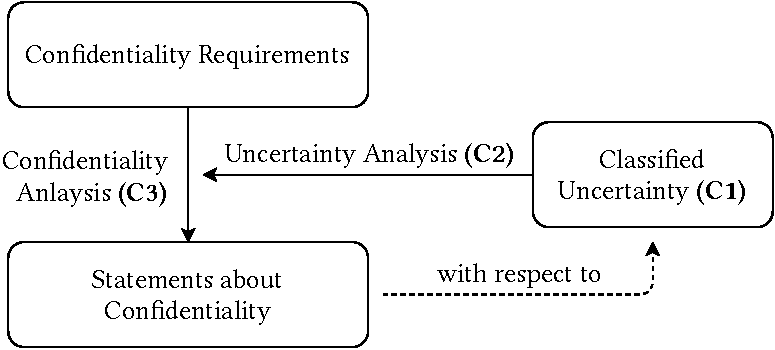
\includegraphics[width=0.75\textwidth]{figures/chapter1/approach.pdf}
    \caption{Schematic and informal visualization of the presented approach.}
    \label{fig:introduction:approach}
\end{figure}

\paragraph{Classifying Uncertainty}
Classifying uncertainty provides the required terminology to inspect and assess uncertainty regarding confidentiality.
By identifying relevant uncertainty types and grouping uncertainty sources into classes, we bootstrap the further analysis process.
This part also includes considering the identification of uncertainty sources by addressing the lack of awareness and expert knowledge of software architects.
Put simply, we first have to investigate the nature of the problem before developing a solution.
This represents an answer to \RQ{1} and also our first Contribution \C{1}.


\paragraph{Uncertainty Analysis}
We build on these findings on the types and attributes of uncertainty sources that affect the confidentiality of a software system to develop an analysis of uncertainty.
Here, we first define an impact analysis to propagate uncertainty.
Based on the relations of the elements of a software architecture, we propagate the effects of uncertainty sources on confidentiality through the architectural model.
Comparable to change impact analysis \cite{heinrich_methodology_2018,busch_architecture-based_2020,rostami_architecture-based_2015}, this analysis yields an impact set that predicts the potential impact of unanticipated change, i.e., uncertainty.
This does not only serve software architects as an early prediction but also shows the effects of uncertainty sources that can subsequently be used in confidentiality analysis.
Put simply, we have to analyze uncertainty first before analyzing confidentiality under uncertainty.
This represents an answer to \RQ{2} and also our second Contribution \C{2}.


\paragraph{Confidentiality Analysis}
Confidentiality analyses take confidentiality requirements as input to make statements about the confidentiality of a software architecture, see \autoref{fig:introduction:approach}.
Based on our previous findings, we extend existing analysis approaches \cite{seifermann_detecting_2022,boltz_extensible_2024} to consider uncertainty.
Here, black-box \cite{walter_architectural_2022} and white-box \cite{hahner_model-based_2023} analysis extensions are possible.
After software architects have modeled sources of uncertainty as part of the architecture model, the uncertainty analysis determines which confidentiality requirements are violated due to which uncertainties.
Here, considering multiple interacting uncertainty sources is especially challenging, as their effects can add up or cancel each other out \cite{camara_uncertainty_2022,camara_addressing_2022}.
This represents an answer to \RQ{3} and also our third Contribution \C{3}.

As discussed previously, all contributions can be used independently or in conjunction.
We also provide tooling that supports the modeling and the analysis based on established frameworks \cite{reussner_modeling_2016,reussner_palladio_2024}.
In this thesis, we motivate, present, and evaluate all contributions independently.
We transparently enumerate assumptions and limitations.
Last, we provide a comprehensive data set including our tooling and all raw evaluation data \cite{dataset}.




\section{Outline and Reading Paths}%
\label{sec:introduction:outline}

This dissertation consists of four parts: The prolog, the contributions, their validation, and the epilog.
The remainder of the prolog comprises the presentation of foundations in \autoref{ch:foundations} and the introduction of a running example in \autoref{ch:runningexample}.
This running example does not only serve to exemplify the scientific problems addressed in this thesis, but will also be used intensively throughout the thesis.
Afterward, we present the contributions of this dissertation.
We start with an overview that continues the introduction of our approach in \autoref{ch:overview}.
Then, we introduce our classification of uncertainty (\C{1}) in \autoref{ch:classification}, the uncertainty impact analysis (\C{2}) in \autoref{ch:impactanalysis}, and four uncertainty-aware confidentiality analysis approaches (\C{3}) in \autoref{ch:confidentialityanalysis}.
We show the scenarios used in the validation of the contributions in \autoref{ch:evaluationscenarios} and present our comprehensive evaluation thereafter in \autoref{ch:evaluation}.
Last, the epilog concludes this thesis with an overview of related work in \autoref{ch:relatedwork} and a summary and outlook on future work in \autoref{ch:conclusion}.
We would also like to point out the additional information in the \hyperref[ch:appendix]{Appendix} and in the data set \cite{dataset}.
There are multiple ways to read this dissertation:

\begin{itemize}
    \item[\faChevronCircleRight] \textbf{Beginner readers}, who are not interested in the technical details of the contributions but want to understand the bigger picture, continue with reading the foundations in \autoref{ch:foundations}.
    Afterward, every chapter ends with a section called \emph{In Simpler Words}.
    There, we explain the most important concepts and findings of each chapter without using scientific terminology but with reference to everyday life.
    For your convenience, this means Sections \ref{sec:introduction:simple}, \ref{sec:foundations:simple}, \ref{sec:runningexample:simple}, \ref{sec:overview:simple}, \ref{sec:classification:simple}, \ref{sec:impactanalysis:simple}, \ref{sec:confidentialityanalysis:simple}, \ref{sec:evaluationscenarios:simple}, \ref{sec:evaluation:simple}, \ref{sec:relatedwork:simple}, and \ref{sec:conclusion:simple}\footnote{%
    This dissertation is meant to be read digitally.
    We make extensive use of references, e.g., between chapters or enumerable items like research questions, contributions, and evaluation goals.
    We recommend using a shortcut to jump back from following a reference.
    Furthermore, all paragraphs, figures, and tables are optimized for the DIN A4 version of this dissertation.
    If you happen to have the DIN A5 or the book version at hand, you can find the other versions until the link expires at \url{https://thesis.abunai.dev/}.}.

    \item[\faChevronCircleRight] \textbf{Expert readers}, who want to gain an overview of our insights, will find gray highlighted boxes titled \emph{Findings} throughout the thesis.
    A concise yet technical overview of the contributions is given in \autoref{ch:overview}, and the conclusion in \autoref{ch:conclusion} provides a summary.
    If the information provided there is not sufficient, the contribution chapters \ref{ch:classification}, \ref{ch:impactanalysis}, and \ref{ch:confidentialityanalysis} come with their own introduction and summary sections.

    \item[\faChevronCircleRight] \textbf{Particularly interested readers} are welcome to read the entire work in one piece.
    Furthermore, we recommend suitable basic literature in \autoref{ch:foundations} and provide all relevant references to own publications at the beginning of each chapter.
\end{itemize}





\section{Summary and Outlook}%
\label{sec:introduction:summary}

In this chapter, we introduced the topic of this thesis.
First, we motivated the actuality and relevance of confidentiality, uncertainty, and software architecture.
Without considering uncertainty as a first-class concern within the software architecture, the validity of statements about confidentiality can be degraded or completely voided \cite{hahner_dealing_2021}.
Afterward, we presented three challenges of architecture-based and uncertainty-aware confidentiality analysis.
They revolve around understanding the relationship between uncertainty and confidentiality, representing uncertainty in architectural models, and providing automated analyses. 
The challenges of representing and analyzing uncertainty in the software architecture are also supported by the literature \cite{troya_uncertainty_2021,hezavehi_uncertainty_2021}.
We summarized these challenges in our problem statement as \emph{inspection problem} (\PR{0}{1}) and \emph{assessment problem} (\PR{0}{2}).

Based on these problems, we presented our research goal and three research questions that map to the three Contributions \C{1} -- \C{3} of this dissertation.
First, we define a novel classification of uncertainty regarding confidentiality.
Second, we use this classification in uncertainty impact analysis, thereby propagating the effects of uncertainty within the software architecture and calculating the potential impact.
Third, we include the impact of uncertainty within confidentiality analysis to identify confidentiality violations with respect to uncertainty.
We summarized the relations of these research questions and our contributions by introducing this dissertation's approach.
Last, we presented the outline and the intended reading paths for the different types of readers of this thesis.

Next, in \readingpath{ch:foundations}, we explain the foundations required for understanding this thesis, e.g., \acp{DAG}, or \ac{MDSD}.
Afterward, we introduce the running example of this thesis in \readingpath{ch:runningexample}.
Both chapters also help to understand the context and the general assumptions of this dissertation.
In \readingpath{ch:overview}, we continue the presentation of our approach by relating common activities in the procedure of handling uncertainty in software architectures to our contributions and our tool support.





\section{In Simpler Words}%
\label{sec:introduction:simple}

Our world runs on data.
Think of social media, online shopping, advertisement, smart home, or artificial intelligence---all of these systems require large amounts of data to provide their functionality.
In this dissertation, we focus on the confidentiality of this data.
Confidentiality demands that data is not shown to unauthorized persons or organizations.
It is a quality property of software systems and is related to security and privacy.
In this dissertation, we research how to analyze the confidentiality of software systems while considering uncertainty.
Put simply, uncertainty is the lack of knowledge, i.e., not knowing something for sure, e.g., because an engineer cannot assess environmental conditions or the behavior of third parties.

We present an approach to better understand the potential impact of uncertainty on confidentiality by using a high-level view of the software system, i.e., software architecture, the big picture of a software system.
Therefore, we first have to better understand uncertainty---like you need to understand the rules of a board game to be able to play better.
Afterward, we build an analysis that propagates uncertainty within a software architecture to better understand its impact.
This is comparable to introducing a drop of dye into a stream of water and then observing the coloration.
In the end, we enable software architects to identify confidentiality violations early and to build better software systems that protect the data of their users.
